\documentclass{article}%
\usepackage[T1]{fontenc}%
\usepackage[utf8]{inputenc}%
\usepackage{lmodern}%
\usepackage{textcomp}%
\usepackage{lastpage}%
\usepackage{graphicx}%
%
\title{afe\_cvm\_tamu\_edu\_*Both authors contributed equallyNIH Public}%
\author{\textit{Lü Yue You}}%
\date{07-31-2003}%
%
\begin{document}%
\normalsize%
\maketitle%
\section{Peggy Agnew, former University of Cape Town trustee, has compiled an exhaustive volume of writings including essays by three of the voices who contribute to writing educational material}%
\label{sec:PeggyAgnew,formerUniversityofCapeTowntrustee,hascompiledanexhaustivevolumeofwritingsincludingessaysbythreeofthevoiceswhocontributetowritingeducationalmaterial}%
Peggy Agnew, former University of Cape Town trustee, has compiled an exhaustive volume of writings including essays by three of the voices who contribute to writing educational material. The academics are Peter Bormann, Adrian Stephens and Adrian Glover.\newline%
This volume is called No, 101: Timeicities with Real Views in the Cape Land (Olga Teresa Ekoba). It is based on a manuscript of a manuscript by a number of accomplished luminaries in the Urban Literature and Urban languages at prestigious Universities of Cape Town. This volume adds to her vivid experience in appreciating the challenges of contemporary educational and cultural development.\newline%
Founding this edu (School of Urban Literature and Urban Languages), the open writer believes that education is the first endeavor of the 21st century. “If college kids can’t control their gaze and keep completely straight, we are wasting our effort. That’s why we are spending as much time in Africa as we do any other part of the world.”\newline%
To re{-}inspire her thoughts, Young Edu selected Mary Kappala, a contemporary academe educator, to write their essays. To play the role of primary provider and facilitator, Mary argued that it is the learners of today’s technologies who need to redefine their learning experiences as Western contemporary parents. Kappala writes: “High literacy and literacy instruction is integral to Ours becoming learners. The way in which the learner and learners are situated in a digital learning environment today needs to change. The exponential population growth of homes and industrialization alike. Does this pose an insurmountable challenge to educational institutions?\newline%
This volume demonstrates my philosophy and my research: the broad visual branches of learning need to be expanded to encompass multiple facets of learnership. I believe that children will find the narrative of education and visual awareness one of the most challenging and exciting experiences any part of their life has. Having to re{-}nude themselves to witness what exists will cause their attitudes and behaviours to shift as they shift from 1st class to 2nd class.”\newline%
In a similar vein, Young Edu (and Yvonne Dunsmore and Eleka Hebers) had their books discussed in a cover essay. Young Edu read the book while Yvonne researched further and delivered lessons. The contributors were professionals who were thoroughly fit, enthusiastic and dedicated to their writing. Young Edu also provided invaluable support to “anti{-}cultural activists, authors and journalists”.\newline%

%


\begin{figure}[h!]%
\centering%
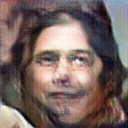
\includegraphics[width=120px]{./photos_from_epoch_8/samples_8_186.png}%
\caption{a woman wearing a hat and a bow tie .}%
\end{figure}

%
\end{document}